% MiniWorld 0 — technical report.  Build:  tectonic docs/paper/main.tex
\documentclass[11pt]{article}

\usepackage[letterpaper,top=1.15in,bottom=1.2in,left=1.35in,right=1.35in]{geometry}
\usepackage{amsmath}
\usepackage{libertinus}
\usepackage{microtype}
\usepackage{graphicx}
\usepackage{booktabs}
\usepackage{tabularx}
\usepackage{enumitem}
\usepackage{titlesec}
\usepackage{tcolorbox}
\usepackage{fancyhdr}
\usepackage[font=small,labelfont={sf,bf},labelsep=period,
            justification=raggedright,singlelinecheck=false]{caption}
\usepackage{xcolor}
\usepackage{tikz}
\usetikzlibrary{arrows.meta,positioning,calc,fit,backgrounds,decorations.pathreplacing}
\usepackage[numbers,sort&compress]{natbib}
\usepackage{hyperref}

% ---------------------------------------------------------------- palette
% One accent hue, used only for structure: section headings, caption labels,
% kickers and links. The wordmark itself stays black -- the numeral in
% "MiniWorld 0" must read as part of the name, not as a highlight.
\definecolor{accent}{HTML}{1F5673}
\definecolor{accentsoft}{HTML}{EEF3F6}
\definecolor{rule}{HTML}{C9D6DE}
\definecolor{muted}{HTML}{5A6B75}
\hypersetup{colorlinks=true, allcolors=accent, citecolor=accent,
            linkcolor=accent, urlcolor=accent}

% ---------------------------------------------------------------- headings
\titleformat{\section}{\sffamily\large\bfseries\color{accent}}{\thesection}{0.7em}{}[\vspace{2pt}\color{rule}\hrule height 0.6pt]
\titleformat{\subsection}{\sffamily\normalsize\bfseries\color{accent!85!black}}{\thesubsection}{0.6em}{}
\titlespacing{\section}{0pt}{1.6\baselineskip}{0.7\baselineskip}
\titlespacing{\subsection}{0pt}{1.0\baselineskip}{0.35\baselineskip}

% ---------------------------------------------------------------- footer
\pagestyle{fancy}\fancyhf{}
\renewcommand{\headrulewidth}{0pt}
\fancyfoot[L]{\sffamily\footnotesize\color{muted}MiniWorld~0 \textperiodcentered\ Technical Report}
\fancyfoot[R]{\sffamily\footnotesize\color{muted}\thepage}

\captionsetup{labelfont={sf,bf,color=accent}}
\setlist[itemize]{leftmargin=1.2em, itemsep=2pt, topsep=3pt}
% Drafting aid, not design: red italic so unfinished spots cannot be missed
% in a proof read. Redefine to {} to hide them all for a clean draft.
\definecolor{draft}{HTML}{C0392B}
\newcommand{\todo}[1]{{\color{draft}\itshape\small[#1]}}
% Name: space-separated numeral, always black. The accent hue is reserved
% for structure (headings/labels/links); colouring the "0" made it read as a
% highlight rather than as part of the wordmark.
% \mw in prose keeps the name unbreakable across lines.
\newcommand{\mw}{MiniWorld~0}
\newcommand{\mwdisplay}{\mbox{MiniWorld 0}}
\definecolor{figaccent}{HTML}{2E86AB}
\definecolor{figsoft}{HTML}{EAF4FA}
% ---------------------------------------------------------------- diagram keys
% The schematics run brighter than the body: pale fills with a saturated
% stroke read as light cards rather than grey slabs. `accentdeep` is the
% body accent, kept for panel titles and counts so the figures still belong
% to this document.
% Boxes are deliberately roomy: \scriptsize text on 4.2pt padding, 10mm tall.
\tikzset{
  op/.style    ={draw=figaccent, line width=0.7pt, fill=figsoft, rounded corners=2.2pt,
                 align=center, font=\scriptsize, inner sep=4.2pt, minimum height=10mm},
  mod/.style   ={op, text width=1.92cm, minimum height=12.5mm},
  wide/.style  ={mod, text width=5.35cm},
  ghost/.style ={draw=rule, line width=0.7pt, dashed, dash pattern=on 2pt off 2pt,
                 fill=none, rounded corners=2.2pt, align=center, font=\scriptsize,
                 inner sep=4.2pt, text width=1.92cm, minimum height=12.5mm, text=muted},
  fl/.style    ={draw=figaccent, line width=0.75pt, -{Stealth[length=4.2pt,width=3.4pt]}},
  gl/.style    ={draw=rule, line width=0.75pt},
  thin/.style  ={draw=muted, line width=0.5pt, densely dotted,
                 -{Stealth[length=3.4pt,width=2.8pt]}},
  res/.style   ={circle, draw=figaccent, line width=0.65pt, fill=white, inner sep=0pt,
                 minimum size=3.4mm, font=\scriptsize},
  fused/.style ={circle, draw=figaccent, line width=0.65pt, fill=figaccent!30, inner sep=0pt,
                 minimum size=3.2mm, font=\scriptsize},
  w/.style     ={font=\scriptsize, text=muted, inner sep=2pt},
  tag/.style   ={font=\small, text=muted, inner sep=2pt},
  cnt/.style   ={font=\small, text=accent, inner sep=2pt},
  ttl/.style   ={font=\small\sffamily\bfseries, text=accent},
  brc/.style   ={decorate, decoration={brace, amplitude=4.5pt, raise=2pt},
                 draw=rule, line width=0.7pt},
}
\newcommand{\pl}{\raisebox{-0.10ex}{$\scriptscriptstyle +$}}

% One AF3-style trimul chain: #1 name prefix, #2 y offset, #3 contraction.
% Every arrow targets a node ANCHOR, never the node centre -- targeting the
% centre buries the arrowhead inside the (+) circle.
\newcommand{\chain}[3]{
  \node[op] (#1LNa) at (1.20,#2)  {LN};
  \node[op] (#1gp)  at (4.15,#2)  {gated\\projection};
  \node[op] (#1ct)  at (7.90,#2)  {$\textstyle\sum_k$ #3};
  \node[op] (#1LNb) at (11.05,#2) {LN};
  \node[op] (#1gp2) at (13.75,#2) {gated\\projection};
  \node[res] (#1pp) at (15.45,#2) {\pl};
  \draw[fl] (-0.55,#2) -- (#1LNa.west);
  \draw[fl] (#1LNa.east) -- (#1gp.west);
  \draw[fl] (#1gp.east)  -- (#1ct.west);
  \draw[fl] (#1ct.east)  -- (#1LNb.west);
  \draw[fl] (#1LNb.east) -- (#1gp2.west);
  \draw[fl] (#1gp2.east) -- (#1pp.west);
  \draw[fl] (#1pp.east)  -- (16.20,#2);
  % the output gate reads the normalised input, not the contraction
  \draw[thin,rounded corners=3pt] ($(#1LNa.east)+(0.22,0)$) -- ++(0,-0.95)
        -| ($(#1gp2.south)+(-0.42,0)$);
  \node[w,anchor=south] at (6.05,#2+0.12) {$a,b$: $2c$};
  \node[w,anchor=south] at (9.50,#2+0.12) {$c$};
}

\newcommand{\kicker}[1]{{\sffamily\footnotesize\bfseries\color{accent}\MakeUppercase{#1}}}

\begin{document}
\thispagestyle{fancy}

% ---------------------------------------------------------------- title
\begingroup
\raggedright
\kicker{Technical Report}\\[0.9em]
{\sffamily\bfseries\fontsize{27}{31}\selectfont \mwdisplay}\\[0.45em]
{\large\color{muted} A compact all-atom biomolecular structure predictor}\\[1.1em]
{\color{rule}\rule{\linewidth}{1.2pt}}\\[0.9em]
{\normalsize Sanggeun Park\textsuperscript{1},\;
\todo{co-authors},\;
Minkyung Baek\textsuperscript{1,\,\textdagger}}\\[0.5em]
{\footnotesize\color{muted}\textsuperscript{1}\,Seoul National University
\hfill Generation 0 \textperiodcentered\ Version 0.1 \textperiodcentered\ \today}\\[0.2em]
{\footnotesize\color{muted}\textsuperscript{\textdagger}\,Corresponding author:
Minkyung Baek \todo{email}}
\endgroup
\vspace{1.4em}

% ---------------------------------------------------------------- abstract
\begin{tcolorbox}[colback=accentsoft, colframe=accentsoft, boxrule=0pt,
  left=1.1em, right=1.1em, top=0.9em, bottom=0.9em, arc=2pt]
{\kicker{Summary}}\\[0.5em]
\todo{One paragraph: what \mw{} is, the staged recipe, headline FoldBench
numbers, what it is for.}
\end{tcolorbox}
\vspace{0.6em}

% ---------------------------------------------------------------- body
\section{Overview}
All-atom structure prediction for arbitrary biomolecular assemblies ---
proteins together with nucleic acids, ligands, ions and covalent modifications
--- was established by AlphaFold~3 \citep{af3} and has since been reproduced by
several open systems \citep{protenix, boltz1, chai1, opendde}. These systems
have converged on a common design: a pair-centric trunk that integrates
sequence, multiple sequence alignments and templates, followed by a diffusion
decoder that generates atomic coordinates directly.

They have not converged on an affordable way to \emph{train} that design.
AlphaFold~3 reports training on 256 A100 GPUs over approximately twenty days
\citep{af3}; among the open systems, Protenix reports 192 GPUs for about two
weeks \citep{protenix}, Boltz-2 reports 128 A100s \citep{boltz2}, ESMFold2
reports 256 H100s for 127 hours \citep{esmfold2}, and OpenDDE reports
$\approx$414{,}000 GPU-hours outright \citep{opendde}. The absolute figures are
not directly comparable, as device generation, crop schedule and dataset size
differ; what they share is a budget of order $10^{4}$--$10^{5}$ GPU-hours
(Table~\ref{tab:compute}), which is beyond the standing allocation of a typical
academic laboratory. Fine-tuning a released checkpoint avoids that cost, but
only for questions the released model was already trained to answer: new
training data, a modified objective, or a changed architecture reinstates the
cost of training in full.

We therefore treat training cost, rather than accuracy on a fixed benchmark, as
the primary design constraint. \mw{} is a compact all-atom predictor trained
under that constraint, in $\approx$\textbf{4{,}300 H100-hours} in total on an
opportunistic, preemptible allocation that varied between 1 and 16 GPUs.
Normalising for device generation places this near $10^{4}$ A100-equivalent
hours --- roughly an order of magnitude below the systems above. Three lines of
work account for the reduction, and they organise this report.

\begin{itemize}
  \item \textbf{Architecture reduction} (\S\ref{sec:arch}). Triangle attention
        is removed from the trunk and the two triangular multiplicative updates
        are merged into a single bidirectional operator
        (\S\ref{sec:bidir}) that shares one normalisation, one output gate and
        one residual between the outgoing and incoming directions. At the atom
        level no pair representation is formed at all: inter-atom geometry
        enters through 3D rotary position encoding inside sliding-window
        attention \citep[Alg.~6--9]{esmfold2}, removing the
        $O(L_{\mathrm{atom}}^{2})$ tensor that otherwise dominates memory at an
        8192-atom crop. Training is staged rather than end-to-end, so a single
        module is live in the optimiser at any time.
  \item \textbf{Kernels} (\S\ref{sec:kernels}). The operators that dominate
        trunk runtime --- triangular multiplication, transition, gated
        normalisation --- are implemented as hand-written fused kernels that
        dispatch on tensor shape and GPU architecture, with normalisation,
        gating, dropout and the residual folded into the kernel epilogue. This
        accounts for the larger part of the measured speedup.
  \item \textbf{A complete release} (\S\ref{sec:release}). Kernels, training
        code, the data pipeline and \emph{the processed training databases
        themselves} are released together, so that reproducing or retargeting
        the model does not begin with rebuilding its inputs.
\end{itemize}

The designation \emph{0} marks this model as the baseline of the series rather
than its strongest member; its purpose is to make the questions that follow
cheap to ask.

\begin{table}[t]
\centering\small\sffamily
\caption{\normalfont\rmfamily Reported training cost of comparable efforts.
Figures are as stated by each source; devices differ, so hours are not directly
comparable across rows.}
\label{tab:compute}
\begin{tabularx}{\linewidth}{@{}Xlr@{}}
\toprule
\rmfamily Model & \rmfamily Devices & \rmfamily GPU-hours \\
\midrule
OpenDDE \citep{opendde}        & 400 Ampere, then 64 Hopper & $\approx$414{,}000 \\
AlphaFold 3 \citep{af3}        & 256 A100, $\approx$20 d    & $\approx$123{,}000 \\
Protenix \citep{protenix}      & 192 GPU, $\approx$2 wk     & $\approx$64{,}500 \\
ESMFold2 \citep{esmfold2}      & 256 H100, 127 h            & $\approx$32{,}500 \\
\midrule
\mw{}                          & 1--16 H100, preemptible    & \textbf{$\approx$4{,}300} \\
\bottomrule
\end{tabularx}
\end{table}

\section{Architecture}
\label{sec:arch}
\subsection{Trunk}
\todo{2--3 sentences: atom input embedder, MSA module, pairformer stack,
template stack, recycling.}

\subsection{Bidirectional triangle multiplication}
\label{sec:bidir}
Figure~\ref{fig:block} contrasts the two pairformer blocks and
Fig.~\ref{fig:dataflow} the dataflow inside the pair update itself; the
pseudocode for both operators is given as Fig.~S1 of the supplement.
AlphaFold~2 and~3 update the pair representation with two triangular
multiplicative operators applied in sequence, one contracting over
\emph{outgoing} edges and one over \emph{incoming} edges
\citep[Alg.~12--13]{af3}. The two differ only in which index is contracted, so
they are one algorithm under a two-way branch (written out as
Fig.~S1 of the supplement); what makes them expensive is that each is
nonetheless a self-contained residual block, re-normalising the same pair
tensor, forming its own output gate and writing its own residual. We merge them
into one operator (Fig.~\ref{fig:dataflow}), which
shares the input normalisation, the output normalisation, the output gate and
the residual between the directions, keeping the hidden capacity and the
$O(L^{3})$ contraction unchanged.

The reduction is summarised in Table~\ref{tab:bidir}. It is modest in
arithmetic --- the contraction dominates the FLOP count and is untouched --- but
substantial in the operations that make the operator memory-bound at the crop
sizes we train on: normalisation passes over the $L\times L\times c_z$ pair
tensor drop from four to two, output gating and the residual from two to one,
and the parameter count from $12c_z^{2}$ to $11c_z^{2}$. It also has a
consequence for implementation that matters more than either: because both
directions read one shared normalised input, a single fused
normalisation-and-gated-projection front can feed both contractions, which is
what the kernel of \S\ref{sec:kernels} exploits.

\par\addvspace{1.0em}\noindent\makebox[\linewidth][c]{%
\begin{minipage}{16.6cm}
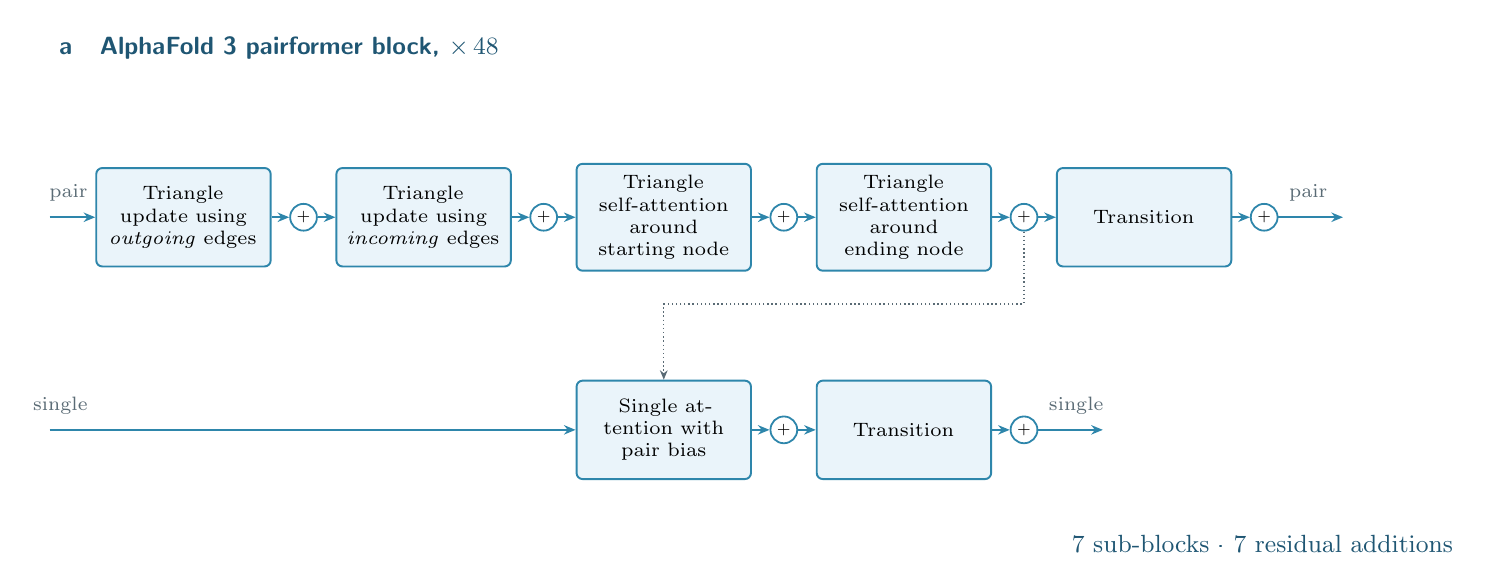
\begin{tikzpicture}[x=1cm,y=1cm]
  \def\dx{3.05}
  \node[ttl,anchor=west] at (-1.70,2.15) {a\quad AlphaFold 3 pairformer block, $\times\,48$};
  \foreach \i/\txt in {0/{Triangle update using \emph{outgoing} edges},
                       1/{Triangle update using \emph{incoming} edges},
                       2/{Triangle self-attention around starting node},
                       3/{Triangle self-attention around ending node},
                       4/{Transition}}
    \node[mod] (p\i) at (\i*\dx,0) {\txt};
  % track labels sit ABOVE their arrows: to the side they collide with the arrow
  \draw[fl] (-1.70,0) -- (p0.west);
  \node[w,anchor=south east] at (-1.14,0.12) {pair};
  \foreach \i in {0,1,2,3}{
    \pgfmathsetmacro{\nx}{int(\i+1)}
    \node[res] (o\i) at (\i*\dx+0.5*\dx,0) {\pl};
    \draw[fl] (p\i.east) -- (o\i.west);
    \draw[fl] (o\i.east) -- (p\nx.west);
  }
  \node[res] (o4) at (4*\dx+0.5*\dx,0) {\pl};
  \draw[fl] (p4.east) -- (o4.west);
  \draw[fl] (o4.east) -- ++(0.82,0);
  \node[w,anchor=south west] at (4*\dx+0.5*\dx+0.24,0.12) {pair};

  \node[mod] (s0) at (2*\dx,-2.70) {Single attention with pair bias};
  \node[mod] (s1) at (3*\dx,-2.70) {Transition};
  \draw[fl] (-1.70,-2.70) -- (s0.west);
  \node[w,anchor=south east] at (-1.14,-2.58) {single};
  \node[res] (q0) at (2*\dx+0.5*\dx,-2.70) {\pl};
  \node[res] (q1) at (3*\dx+0.5*\dx,-2.70) {\pl};
  \draw[fl] (s0.east) -- (q0.west);
  \draw[fl] (q0.east) -- (s1.west);
  \draw[fl] (s1.east) -- (q1.west);
  \draw[fl] (q1.east) -- ++(0.82,0);
  \node[w,anchor=south west] at (3*\dx+0.5*\dx+0.24,-2.58) {single};
  \draw[thin] (o3.south) -- ++(0,-0.92) -| (s0.north);
  \node[cnt,anchor=east] at (16.20,-4.15)
        {7 sub-blocks \textperiodcentered\ 7 residual additions};
\end{tikzpicture}

\vspace{2.6em}

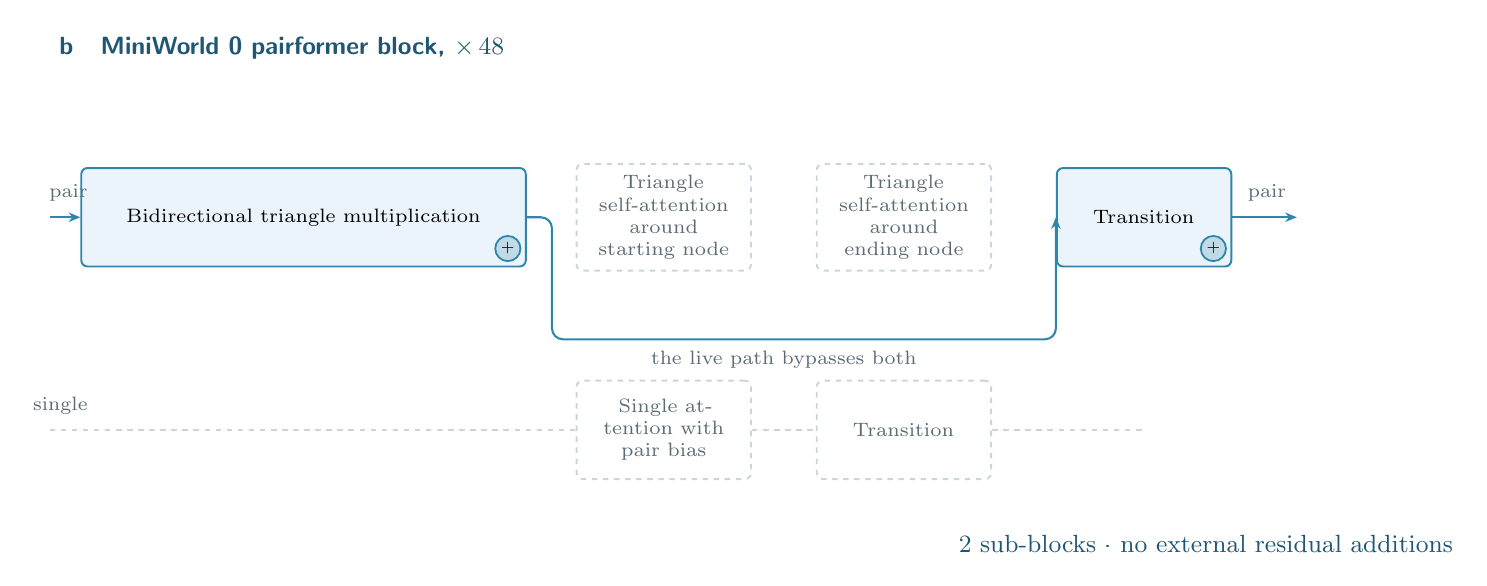
\begin{tikzpicture}[x=1cm,y=1cm]
  \def\dx{3.05}
  \node[ttl,anchor=west] at (-1.70,2.15) {b\quad \mbox{MiniWorld 0} pairformer block, $\times\,48$};
  \node[wide] (b0) at (0.5*\dx,0) {Bidirectional triangle multiplication};
  \node[mod]  (b1) at (4*\dx,0)   {Transition};
  \node[fused] at ($(b0.south east)+(-0.24,0.24)$) {\pl};
  \node[fused] at ($(b1.south east)+(-0.24,0.24)$) {\pl};
  \node[ghost] (g2) at (2*\dx,0) {Triangle self-attention around starting node};
  \node[ghost] (g3) at (3*\dx,0) {Triangle self-attention around ending node};
  \draw[fl] (-1.70,0) -- (b0.west);
  \node[w,anchor=south east] at (-1.14,0.12) {pair};
  % the live path is routed clear beneath the two deleted attentions
  \draw[fl,rounded corners=4pt]
        (b0.east) -- ++(0.32,0) -- ++(0,-1.55)
        -- ($(b1.west)+(-0.32,-1.55)$) -- ($(b1.west)+(0,-1.55)$) -- (b1.west);
  \node[w,anchor=north] at (2.5*\dx,-1.62) {the live path bypasses both};
  \draw[fl] (b1.east) -- ++(0.82,0);
  \node[w,anchor=south west] at (4*\dx+1.24,0.12) {pair};
  \node[ghost] (g4) at (2*\dx,-2.70) {Single attention with pair bias};
  \node[ghost] (g5) at (3*\dx,-2.70) {Transition};
  \draw[gl,dashed,dash pattern=on 2pt off 2pt] (-1.70,-2.70) -- (g4.west);
  \node[w,anchor=south east] at (-1.14,-2.58) {single};
  \draw[gl,dashed,dash pattern=on 2pt off 2pt] (g4.east) -- (g5.west);
  \draw[gl,dashed,dash pattern=on 2pt off 2pt] (g5.east) -- ++(1.95,0);
  \node[cnt,anchor=east] at (16.20,-4.15)
        {2 sub-blocks \textperiodcentered\ no external residual additions};
\end{tikzpicture}

\vspace{1.8em}


\begin{tikzpicture}[x=1cm,y=1cm]
  \node[mod,minimum height=5.4mm,text width=1.05cm] at (0,0) {};
  \node[tag,anchor=west] at (0.78,0) {retained};
  \node[ghost,minimum height=5.4mm,text width=1.05cm] at (3.60,0) {};
  \node[tag,anchor=west] at (4.38,0) {removed};
  \node[res] at (7.40,0) {\pl};
  \node[tag,anchor=west] at (7.68,0) {residual added by the block};
  \node[fused] at (12.30,0) {\pl};
  \node[tag,anchor=west] at (12.58,0) {residual fused into the kernel};
\end{tikzpicture}
\end{minipage}}\par\addvspace{0.5em}
\noindent\makebox[\linewidth][c]{%
\begin{minipage}{16.6cm}\captionof{figure}{The pairformer block of AlphaFold~3 (\emph{a}) and of \mw{}
(\emph{b}), drawn on the same horizontal slots so the panels can be read
column-wise. \mw{} merges the two triangular multiplicative updates into one
bidirectional operator, drops both triangle self-attentions, and carries no
single track in the trunk at all; the live path visibly routes around the
deleted attentions. AlphaFold~3 adds a residual after every sub-block, whereas
in \mw{} each operator applies its own residual inside the kernel epilogue, so
no addition appears on the flow line.}
\label{fig:block}\end{minipage}}\par\addvspace{1.0em}

\par\addvspace{1.1em}
\noindent\begin{center}
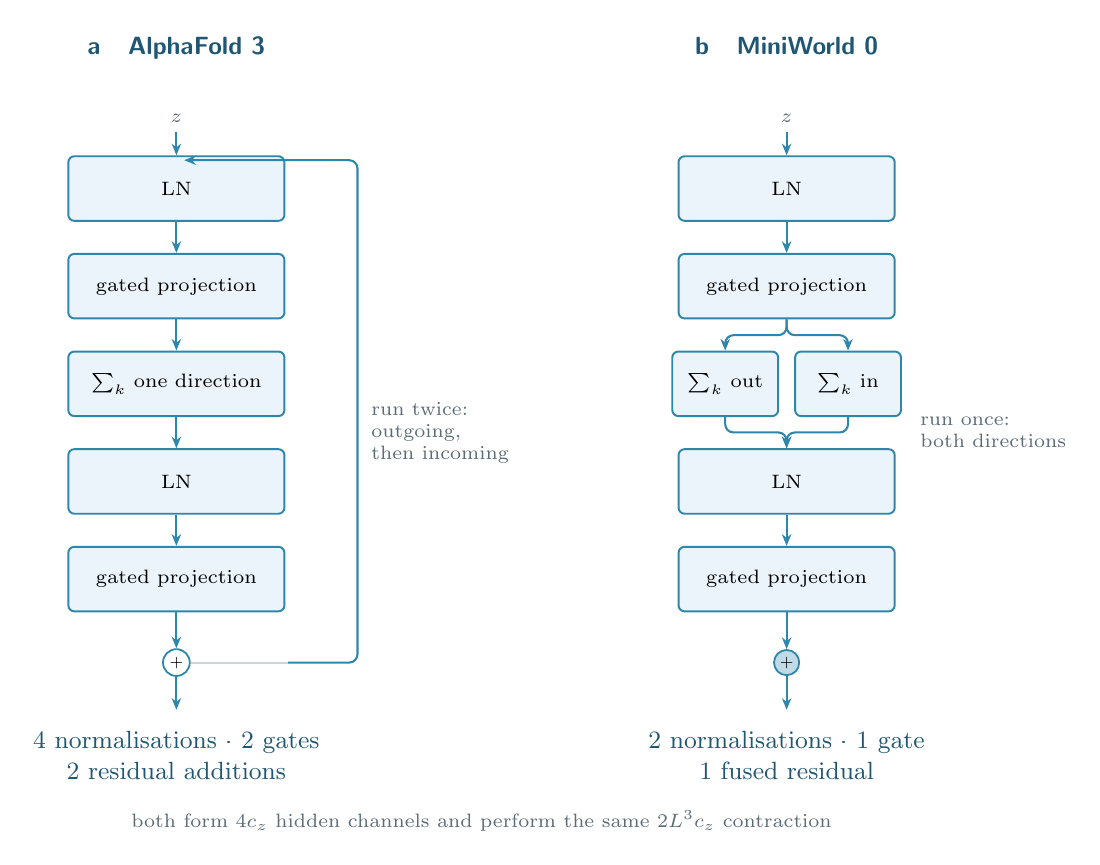
\begin{tikzpicture}[x=1cm,y=1cm]
  % Panels side by side, each a top-to-bottom pass. Drawn this way the two are
  % directly comparable: AlphaFold 3 must run the column twice (the loop), we
  % run it once and split only at the contraction (the fork).
  \tikzset{vop/.style={op, text width=2.45cm, minimum height=8.2mm, font=\scriptsize},
           sop/.style={op, text width=1.05cm, minimum height=8.2mm, font=\scriptsize}}
  \def\pa{0}      % panel a centre
  \def\pb{7.75}   % panel b centre
  \def\dy{1.24}

  \node[ttl,anchor=north] at (\pa,2.05) {a\quad AlphaFold 3};
  \node[ttl,anchor=north] at (\pb,2.05) {b\quad \mbox{MiniWorld 0}};

  % ---------------- panel a: one column, run twice ---------------------------
  \node[vop] (aln1) at (\pa,0)        {LN};
  \node[vop] (agp1) at (\pa,-\dy)     {gated projection};
  \node[vop] (act)  at (\pa,-2*\dy)   {$\textstyle\sum_k$ one direction};
  \node[vop] (aln2) at (\pa,-3*\dy)   {LN};
  \node[vop] (agp2) at (\pa,-4*\dy)   {gated projection};
  \node[res] (app)  at (\pa,-5*\dy+0.18) {\pl};
  \draw[fl] (\pa,0.72) -- (aln1.north);
  \node[w,anchor=south] at (\pa,0.76) {$z$};
  \foreach \u/\v in {aln1/agp1, agp1/act, act/aln2, aln2/agp2} \draw[fl] (\u.south) -- (\v.north);
  \draw[fl] (agp2.south) -- (app.north);
  \draw[fl] (app.south) -- (\pa,-5*\dy-0.42);
  % the loop: the whole column is executed once per direction
  \draw[fl,rounded corners=3pt] (\pa+1.42,-5*\dy+0.18) -- (\pa+2.30,-5*\dy+0.18)
        -- (\pa+2.30,0.36) -- (\pa+0.10,0.36);
  \draw[gl] (app.east) -- (\pa+1.42,-5*\dy+0.18);
  \node[w,anchor=west,align=left] at (\pa+2.40,-2.5*\dy)
        {run twice:\\outgoing,\\then incoming};

  % ---------------- panel b: one column, forked at the contraction -----------
  \node[vop] (bln1) at (\pb,0)        {LN};
  \node[vop] (bgp1) at (\pb,-\dy)     {gated projection};
  \node[sop] (bco)  at (\pb-0.78,-2*\dy) {$\textstyle\sum_k$ out};
  \node[sop] (bci)  at (\pb+0.78,-2*\dy) {$\textstyle\sum_k$ in};
  \node[vop] (bln2) at (\pb,-3*\dy)   {LN};
  \node[vop] (bgp2) at (\pb,-4*\dy)   {gated projection};
  \node[fused] (bpp) at (\pb,-5*\dy+0.18) {\pl};
  \draw[fl] (\pb,0.72) -- (bln1.north);
  \node[w,anchor=south] at (\pb,0.76) {$z$};
  \draw[fl] (bln1.south) -- (bgp1.north);
  \draw[fl,rounded corners=3pt] (bgp1.south) -- ++(0,-0.20) -| (bco.north);
  \draw[fl,rounded corners=3pt] (bgp1.south) -- ++(0,-0.20) -| (bci.north);
  \draw[fl,rounded corners=3pt] (bco.south) |- ($(bln2.north)+(0,0.20)$) -- (bln2.north);
  \draw[fl,rounded corners=3pt] (bci.south) |- ($(bln2.north)+(0,0.20)$) -- (bln2.north);
  \draw[fl] (bln2.south) -- (bgp2.north);
  \draw[fl] (bgp2.south) -- (bpp.north);
  \draw[fl] (bpp.south) -- (\pb,-5*\dy-0.42);
  \node[w,anchor=west,align=left] at (\pb+1.62,-2.5*\dy) {run once:\\both directions};

  % ---------------- counts ---------------------------------------------------
  \node[cnt,anchor=north,align=center] at (\pa,-5*\dy-0.62)
        {4 normalisations \textperiodcentered\ 2 gates\\2 residual additions};
  \node[cnt,anchor=north,align=center] at (\pb,-5*\dy-0.62)
        {2 normalisations \textperiodcentered\ 1 gate\\1 fused residual};
  \node[w,anchor=north] at (0.5*\pb+0.5*\pa,-5*\dy-1.62)
        {both form $4c_z$ hidden channels and perform the same $2L^{3}c_z$ contraction};
\end{tikzpicture}
\end{center}
\par\addvspace{0.3em}
\captionof{figure}{Dataflow inside the pair update, one pass per column.
AlphaFold~3 (\emph{a}) executes the whole column once per direction, so every
normalisation, gate, projection and residual happens twice. \mw{} (\emph{b})
executes it once and splits only at the contraction --- the single place where
the directions differ --- so the front and the back are shared. Hidden capacity
and the $O(L^{3})$ contraction are unchanged; what falls away is the duplicated
$O(L^{2})$ work around them. The shaded $\oplus$ marks a residual folded into
the kernel epilogue (\S\ref{sec:kernels}) rather than added by the caller.}
\label{fig:dataflow}
\par\addvspace{1.0em}


\begin{table}[t]
\centering\small\sffamily
\caption{\normalfont\rmfamily Per-block cost of the pair update, at
AlphaFold~3's setting $c = h = c_z = 128$. Both forms produce $4c_z$ hidden
channels and perform the same $2L^{3}c_z$ contraction multiply--accumulates;
they differ in the surrounding $O(L^{2})$ work.}
\label{tab:bidir}
\begin{tabularx}{\linewidth}{@{}Xcc@{}}
\toprule
\rmfamily & \rmfamily AlphaFold 3 & \rmfamily \mw{} \\
\midrule
LayerNorm passes over the pair tensor & 4 & \textbf{2} \\
Input projection width (total)        & $4c$ & $4h$ \\
\quad issued as                      & 2 GEMMs & \textbf{1 GEMM} \\
Contraction (multiply--accumulates)   & $2L^{3}c$ & $2L^{3}h$ \\
Output projection                     & 2 GEMMs & \textbf{1 GEMM} \\
Output gate                           & 2 GEMMs & \textbf{1 GEMM} \\
Residual additions                    & 2 & \textbf{1} \\
Dropout masks                         & 2 & \textbf{1} \\
Parameters                            & $12c_z^{2}$ & $\mathbf{11}c_z^{2}$ \\
\bottomrule
\end{tabularx}
\end{table}

\subsection{Diffusion module}
The denoiser is trained with the EDM objective \citep{edm} under AlphaFold~3
preconditioning. Atom encoder and decoder are adaLN-Zero blocks \citep{dit}
with sliding-window attention \citep[Alg.~8]{esmfold2}; the token trunk keeps
the pair-biased transformer of AlphaFold~3.

\subsection{Confidence head}
\todo{1--2 sentences: pLDDT / PAE / PDE over the frozen pair representation.}

\begin{table}[t]
\centering\small\sffamily
\caption{\normalfont\rmfamily \mw{} configuration.}
\label{tab:config}
\begin{tabularx}{\linewidth}{@{}Xr@{}}
\toprule
\rmfamily Component & \rmfamily Setting \\
\midrule
Token / pair width                    & 384 / 128 \\
Atom input embedder                   & 3 blocks \\
MSA module                            & 4 blocks \\
Pairformer                            & 48 blocks \\
Diffusion token transformer           & 24 blocks \\
Diffusion atom transformer            & 3 blocks, window 128 \\
Recycling                             & up to 4 \\
Training crop                         & 768 tokens / 8192 atoms \\
Parameters                            & \rmfamily\todo{count} \\
\bottomrule
\end{tabularx}
\end{table}

\section{Kernels}
\label{sec:kernels}
Reducing the architecture lowers the work; kernels decide how much of the
hardware that work actually uses. We treat the fused operations as a
first-class deliverable rather than an implementation detail, and they account
for most of the throughput behind Table~\ref{tab:compute}.

Each operation is a complete, autograd-transparent unit that takes its weights
as arguments and selects a backend internally, per tensor shape and per GPU
architecture. A caller asks for \emph{ours} and gets whichever hand-written
kernel is fastest and correct on the running device, falling back to a slower
but valid path rather than a wrong one.

\todo{This section is the main selling point --- expand: which ops are fused,
what the fusion is (LN folded into the epilogue, residual fused into the
kernel, dual-B gated collective for trimul), the autotune cache, and a clean
benchmark table re-measured on H100 rather than the development figures below.}

\begin{table}[t]
\centering\small\sffamily
\caption{\normalfont\rmfamily Kernel timings recorded during development.
\todo{re-measure on H100 under one harness before publication}}
\label{tab:kernels}
\begin{tabularx}{\linewidth}{@{}Xrrr@{}}
\toprule
\rmfamily Operation & \rmfamily PyTorch & \rmfamily Triton & \rmfamily Ours \\
\midrule
Triangle multiplication, $L{=}384$ & 1.14 ms & 0.284 ms & \textbf{0.115 ms} \\
Fused LN + mask, $L{=}1024$        & 0.55 ms & ---      & \textbf{0.090 ms} \\
\bottomrule
\end{tabularx}
\end{table}

\section{Training}
\label{sec:training}
Training is staged rather than end-to-end. Each stage loads the previous
stage's checkpoint and freezes every parameter it finds there, so exactly one
module is live in the optimiser at any time; the parameter policy is
declarative (\texttt{default: freeze\_loaded} plus an explicit list of modules
to (re)initialise and train), which is what keeps the stage boundaries honest.
The practical consequence is that no stage ever has to hold optimiser state,
activations and gradients for the whole model, and each stage can be sized to
the hardware that happens to be free.

Table~\ref{tab:stages} gives the recipe and its measured cost. Stages 1 and 2
differ only in crop: the trunk is trained at a 384-token crop until the
distogram loss flattens, then continued at 768 tokens with gradient
checkpointing enabled on all MSA and pairformer blocks, which buys the larger
crop at roughly constant memory. Stage 3 attaches the diffusion module to the
frozen trunk; because the trunk runs under \texttt{no\_grad} it contributes no
backward activations, so the 768-token crop is cheap on the trunk side and the
atom-level denoiser at 48 noise augmentations per example is the memory driver.
Stage 4 trains only the confidence head, reading a structure sampled from the
frozen diffusion module.

All stages share an effective batch of 256, held constant across the GPU ladder
by adjusting gradient accumulation, and use Adam with a 1000-step warmup, a
$5\times10^{4}$-step decay and an exponential moving average of the weights
($\gamma = 0.999$). The allocation is opportunistic: a coordinator submits the
largest ladder size $\{16, 8, 4, 1\}$ that fits the free GPUs, resumes from the
latest checkpoint when the job is preempted, and only upsizes at an epoch
boundary after the extra GPUs have stayed free for three hours. Training was
therefore spread over 134 separate SLURM jobs rather than one reservation,
which is why the hours in Table~\ref{tab:stages} are measured from the logged
step timestamps: the allocation the jobs held is a poor proxy for training,
since a job that is preempted during start-up consumes GPUs without taking a
single step.

\begin{table}[t]
\centering\footnotesize\sffamily
\caption{\normalfont\rmfamily\small Training stages. Settings are given per
stage in the manner of AlphaFold~3's Table~6 \citep{af3}; a dash means the
component is not active in that stage. Epochs are the cumulative counter
carried across stages, and steps and samples are what was actually reached ---
read from the final checkpoint, not from the configured target: at the end of
stage~3 the counter stands at epoch 948 and $94\,800$ optimiser steps, i.e.\ 100
steps per epoch throughout. Hours are \emph{training} hours: every optimiser
step is timestamped in the run logs, and we sum, over every run, the interval
from its first step to its last and multiply by the GPUs it held. Time spent on
process start-up, compilation, dataloader warm-up and preemption before the
first step is therefore excluded. Stage~3's raised learning rate reflects a
frozen trunk and a diffusion head trained from scratch; its hours cover both the
surviving $5\times10^{-3}$ run (638\,h, to epoch 948) and an earlier
$1.8\times10^{-3}$ attempt abandoned at epoch 915 (282\,h). Stage~4 has
not been run yet. Shared across all stages:
effective batch 256, Adam ($\beta_1=0.9$, $\beta_2=0.95$), 1000-step linear
warmup, decay $0.95$ per $5\times10^4$ steps, gradient clipping at global norm
1.0, and an exponential moving average with $\gamma=0.999$. Gradient checkpointing is per block and
applies only to the module being trained: stage~2 checkpoints every MSA (4) and
pairformer (48) block of the trunk, stage~3 every token-DiT (24) and atom-SWA
(3) block of the diffusion module. The frozen trunk in stages~3 and~4 runs
under \texttt{no\_grad} and stores no activations, so it needs none.}
\label{tab:stages}
\begin{tabularx}{\linewidth}{@{}Xcccc@{}}
\toprule
\rmfamily & \rmfamily 1 & \rmfamily 2 & \rmfamily 3 & \rmfamily 4 \\
\midrule
\rmfamily Token crop $N_{\mathrm{token}}$      & 384 & 768 & 768 & 768 \\
\rmfamily Atom crop $N_{\mathrm{atom}}$        & 4{,}096 & 8{,}192 & 8{,}192 & 8{,}192 \\
\rmfamily Parameters initialised from          & random & stage 1 & stage 2 & stage 3 \\
\rmfamily Module trained                       & trunk & trunk & diffusion & confidence \\
\rmfamily Modules frozen                       & --- & --- & trunk & trunk, diffusion \\
\addlinespace[2pt]
\rmfamily Distogram loss weight                & 1 & 1 & --- & --- \\
\rmfamily Diffusion loss weight                & --- & --- & 4 & --- \\
\rmfamily pLDDT / PDE / PAE loss weight        & --- & --- & --- & 1 / 1 / 1 \\
\addlinespace[2pt]
\rmfamily Gradient checkpointing (blocks)      & off & 4 + 48 & 24 + 3 & off \\
\rmfamily Noise augmentations per example      & --- & --- & 48 & --- \\
\rmfamily Diffusion rollout steps              & --- & --- & --- & 200 \\
\rmfamily Base learning rate ($10^{-3}$)       & 1.8 & 1.8 & 5.0 & 1.0 \\
\addlinespace[2pt]
\rmfamily Epochs (cumulative counter)          & 0--800 & 800--900 & 900--948 & --- \\
\rmfamily Optimiser steps in stage ($10^{3}$)  & 80.0 & 10.0 & 4.8 & --- \\
\rmfamily Training samples ($10^{6}$)          & 20.5 & 2.6 & 1.2 & --- \\
\rmfamily \textbf{Training (H100-hours)}       & \textbf{2{,}321} & \textbf{1{,}058} & \textbf{920} & \rmfamily\todo{--} \\
\bottomrule
\end{tabularx}
\end{table}

The clearest read on efficiency comes from stage~1, because it can be matched
against AlphaFold~3's initial training stage on the quantities that matter:
both use a 384-token crop, both use an effective batch of 256, and both run for
essentially the same number of optimiser steps --- $\approx$78{,}000 for
AlphaFold~3 ($\approx$20$\times10^{6}$ samples) against 80{,}000 here
($20.5\times10^{6}$ samples). AlphaFold~3 reports $\approx$10 days on 256
A100s for that stage, or $\approx$61{,}000 A100-hours; stage~1 here took
2{,}321 H100-hours. Allowing a factor of two to three for the device
generation, the same step budget at the same crop and batch size was reached
for roughly nine to thirteen times less compute. The comparison is not
perfectly matched --- AlphaFold~3 trains its trunk, diffusion module and
confidence heads jointly in that stage, whereas stage~1 trains only the trunk
against the distogram loss --- but the crop, the batch and the step count are
held fixed, which the aggregate figures of Table~\ref{tab:compute} do not do.

\section{Data and release}
\label{sec:release}
\todo{BioMol: a data format for biomolecular structures. DataCooker: explicit,
declarative data processing. The released databases. What OpenFold
\citep{openfold} did and what is different here.}

\section{Results}
We evaluate on FoldBench \citep{foldbench}, reporting lDDT \citep{lddt} for
monomers and DockQ \citep{dockqv2} pass rates for interfaces.
\todo{results pending}

\section{Discussion}
\todo{What this enables: the point of a cheap baseline is that ideas become
testable. List the directions this makes affordable.}

\small
\bibliographystyle{unsrtnat}
\bibliography{refs}

\end{document}
